%%%%%%%%%%%%%%%%%%%%%%%%%%%%%%%%%%%%%%%%%
% Programming/Coding Assignment
% LaTeX Template
%
% This template has been downloaded from:
% http://www.latextemplates.com
%
% Original author:
% Ted Pavlic (http://www.tedpavlic.com)
%
% Note:
% The \lipsum[#] commands throughout this template generate dummy text
% to fill the template out. These commands should all be removed when 
% writing assignment content.
%
% This template uses a Perl script as an example snippet of code, most other
% languages are also usable. Configure them in the "CODE INCLUSION 
% CONFIGURATION" section.
%
%%%%%%%%%%%%%%%%%%%%%%%%%%%%%%%%%%%%%%%%%

%----------------------------------------------------------------------------------------
%	PACKAGES AND OTHER DOCUMENT CONFIGURATIONS
%----------------------------------------------------------------------------------------

\documentclass{article}

\usepackage{fancyhdr} % Required for custom headers
\usepackage{lastpage} % Required to determine the last page for the footer
\usepackage{extramarks} % Required for headers and footers
\usepackage[usenames,dvipsnames]{color} % Required for custom colors
\usepackage{graphicx} % Required to insert images
\usepackage{listings} % Required for insertion of code
\usepackage{courier} % Required for the courier font
\usepackage{lipsum} % Used for inserting dummy 'Lorem ipsum' text into the template

\usepackage{tikz}
\usetikzlibrary{arrows} 

\usepackage{quoting}
\quotingsetup{vskip=0pt}

\usepackage{mathtools}
\usepackage{amsmath, amsthm, amssymb}
\usepackage[ansinew]{inputenc}

% Margins
\topmargin=-0.45in
\evensidemargin=0in
\oddsidemargin=0in
\textwidth=6.5in
\textheight=9.0in
\headsep=0.25in

\linespread{1.1} % Line spacing

% Set up the header and footer
\pagestyle{fancy}
\lhead{\hmwkAuthorName} % Top left header
\chead{\hmwkClass: \hmwkTitle} % Top center head
\rhead{}
\cfoot{} % Bottom center footer
\rfoot{Page\ \thepage\ of\ \protect\pageref{LastPage}} % Bottom right footer
\renewcommand\headrulewidth{0.4pt} % Size of the header rule
\renewcommand\footrulewidth{0.4pt} % Size of the footer rule

\setlength\parindent{0pt} % Removes all indentation from paragraphs

%----------------------------------------------------------------------------------------
%	CODE INCLUSION CONFIGURATION
%----------------------------------------------------------------------------------------

\definecolor{MyDarkGreen}{rgb}{0.0,0.4,0.0} % This is the color used for comments
\lstloadlanguages{Perl} % Load Perl syntax for listings, for a list of other languages supported see: ftp://ftp.tex.ac.uk/tex-archive/macros/latex/contrib/listings/listings.pdf
\lstset{language=Perl, % Use Perl in this example
        frame=single, % Single frame around code
        basicstyle=\small\ttfamily, % Use small true type font
        keywordstyle=[1]\color{Blue}\bf, % Perl functions bold and blue
        keywordstyle=[2]\color{Purple}, % Perl function arguments purple
        keywordstyle=[3]\color{Blue}\underbar, % Custom functions underlined and blue
        identifierstyle=, % Nothing special about identifiers                                         
        commentstyle=\usefont{T1}{pcr}{m}{sl}\color{MyDarkGreen}\small, % Comments small dark green courier font
        stringstyle=\color{Purple}, % Strings are purple
        showstringspaces=false, % Don't put marks in string spaces
        tabsize=5, % 5 spaces per tab
        %
        % Put standard Perl functions not included in the default language here
        morekeywords={rand},
        %
        % Put Perl function parameters here
        morekeywords=[2]{on, off, interp},
        %
        % Put user defined functions here
        morekeywords=[3]{test},
       	%
        morecomment=[l][\color{Blue}]{...}, % Line continuation (...) like blue comment
        numbers=left, % Line numbers on left
        firstnumber=1, % Line numbers start with line 1
        numberstyle=\tiny\color{Blue}, % Line numbers are blue and small
        stepnumber=5 % Line numbers go in steps of 5
}

% Creates a new command to include a perl script, the first parameter is the filename of the script (without .pl), the second parameter is the caption
\newcommand{\perlscript}[2]{
\begin{itemize}
\item[]\lstinputlisting[caption=#2,label=#1]{#1.pl}
\end{itemize}
}

%----------------------------------------------------------------------------------------
%	DOCUMENT STRUCTURE COMMANDS
%	Skip this unless you know what you're doing
%----------------------------------------------------------------------------------------

% Header and footer for when a page split occurs within a problem environment
\newcommand{\enterProblemHeader}[1]{
\nobreak\extramarks{#1}{#1 continued on next page\ldots}\nobreak
\nobreak\extramarks{#1 (continued)}{#1 continued on next page\ldots}\nobreak
}

% Header and footer for when a page split occurs between problem environments
\newcommand{\exitProblemHeader}[1]{
\nobreak\extramarks{#1 (continued)}{#1 continued on next page\ldots}\nobreak
\nobreak\extramarks{#1}{}\nobreak
}

\setcounter{secnumdepth}{0} % Removes default section numbers
\newcounter{homeworkProblemCounter} % Creates a counter to keep track of the number of problems

\newcommand{\homeworkProblemName}{}
\newenvironment{homeworkProblem}[1][Question \arabic{homeworkProblemCounter}]{ % Makes a new environment called homeworkProblem which takes 1 argument (custom name) but the default is "Problem #"
\stepcounter{homeworkProblemCounter} % Increase counter for number of problems
\renewcommand{\homeworkProblemName}{#1} % Assign \homeworkProblemName the name of the problem
\section{\homeworkProblemName} % Make a section in the document with the custom problem count
\enterProblemHeader{\homeworkProblemName} % Header and footer within the environment
}{
\exitProblemHeader{\homeworkProblemName} % Header and footer after the environment
}

\newcommand{\problemAnswer}[1]{ % Defines the problem answer command with the content as the only argument
\noindent\framebox[\columnwidth][c]{\begin{minipage}{0.98\columnwidth}#1\end{minipage}} % Makes the box around the problem answer and puts the content inside
}

\newcommand{\homeworkSectionName}{}
\newenvironment{homeworkSection}[1]{ % New environment for sections within homework problems, takes 1 argument - the name of the section
\renewcommand{\homeworkSectionName}{#1} % Assign \homeworkSectionName to the name of the section from the environment argument
\subsection{\homeworkSectionName} % Make a subsection with the custom name of the subsection
\enterProblemHeader{\homeworkProblemName\ [\homeworkSectionName]} % Header and footer within the environment
}{
\enterProblemHeader{\homeworkProblemName} % Header and footer after the environment
}

%----------------------------------------------------------------------------------------
%	NAME AND CLASS SECTION
%----------------------------------------------------------------------------------------

\newcommand{\hmwkTitle}{Assignment\ \#1} % Assignment title
\newcommand{\hmwkDueDate}{Friday, 16\textsuperscript{th} of May, 2016} % Due date
\newcommand{\hmwkClass}{Design and Analysis of Algorithms} % Course/class
\newcommand{\hmwkClassTime}{4:00pm} % Class/lecture time
\newcommand{\hmwkClassInstructor}{Jones} % Teacher/lecturer
\newcommand{\hmwkAuthorName}{Tim Cochrane} % Your name
\newcommand{\studentNum}{17766247}

%----------------------------------------------------------------------------------------
%	TITLE PAGE
%----------------------------------------------------------------------------------------

\title{
\vspace{2in}
\textmd{\textbf{\hmwkClass}}\\
\textmd{\hmwkTitle}\\
\normalsize\vspace{0.1in}\small{\hmwkDueDate}\\
\vspace{3in}
}

\author{\textbf{\hmwkAuthorName} \\ \studentNum}
\date{} % Insert date here if you want it to appear below your name

%----------------------------------------------------------------------------------------

\begin{document} 
\maketitle\thispagestyle{empty}

%----------------------------------------------------------------------------------------
%	TABLE OF CONTENTS
%----------------------------------------------------------------------------------------

%\setcounter{tocdepth}{1} % Uncomment this line if you don't want subsections listed in the ToC

%  \newpage
%  \tableofcontents
%  \newpage

\clearpage
\setcounter{page}{1}

%----------------------------------------------------------------------------------------
%	PROBLEM 1
%----------------------------------------------------------------------------------------

% To have just one problem per page, simply put a \clearpage after each problem

\begin{homeworkProblem}

    a) Use the Master method solve the folloing recurrence function:
    \begin{center}
        $T(n) = 3T(\sqrt[2]{n}) + \log_2{n}$
    \end{center}
    \textbf{Solution}
    \begin{quoting}
        \abovedisplayskip=0pt
        \begin{align}
            \shortintertext{Inital recurance:}
            T(n) & = 3T(\sqrt[2]{n}) + \log_2{n} \notag \\
            \shortintertext{Substitute for $k = \log_2{n}$:}
            T(2^k) & = 3T(2^{\frac{k}{2}}) + k \notag \\
            \shortintertext{Now in the master thereom form:}
            T(n) & = aT(n/b) + f(n) \notag \\
            \shortintertext{Where:}
            a = 3, b & = 2, f(n) = k \notag
            \shortintertext{Checking which master thereom case to use:}
            k^{\log_b{a}} & = k^{\log_2{3}} \approx k^{1.6} \notag \\
            k^{1} & < k^{1.6} \notag
        \end{align}
        \begin{center}
            $\therefore$ case 1 of master thereom \\
            The solution to the recurance is $O(n^{\log_2{3}})$.
        \end{center}
    \end{quoting}
    \vskip0.5cm
   %\begin{align}
   %    \sqrt{k} = \sqrt{\log_2{n}} = 2^{\frac{\log_2{n}}{2}} = 2^\frac{k}{2}
   %\end{align}

    b) Consider the recurrence function $T(n) = 2T(n-1)+1$ state the upper 
    bound time complexity of the function and use induction to 
    prove that the time complexity is correct. \\

    \textbf{Solution}

    \begin{quoting}
        Assuming that $T(1) = 1$ lets calculate the first few values of the
        the recurrance to get an idea of the function.
        \begin{align}
            T(1) & = 1 \notag \\
            T(2) & = 2(1) + 1 = 3 \notag \\
            T(3) & = 2(3) + 1 = 7 \notag \\
            T(4) & = 2(7) + 1 = 15 \notag
        \end{align}

        The initial values of the recurrance appears to be $2^{n} - 1$. Lets
        try and prove this by induction. \\

        \textbf{Inductive Hypothesis}
        \begin{center}
            $T(n) \in O(2^{n} - 1)$
        \end{center}
        \textbf{Base Case}
        \begin{align}
            T(2) & = 2T(2 - 1) + 1 & 2^{2} - 1 & = 4 - 1 \notag \\
                 & = 2T(1) + 1 & & = 3 \notag \\
                 & = 2 + 1 = 3 & & = 3 \notag
        \end{align}
        \begin{center}
            $\therefore$ \text{base case holds}
        \end{center}

        \textbf{Inductive Step}
        \begin{align}
            T(n + 1) & = 2T(n + 1 - 1) + 1 \notag \\
                     & = 2T(n) + 1 \notag \\
                     & = 2(2^{n} - 1) + 1 \notag \\
                     & = 2^{n+1} - 2 + 1 \notag \\
                     & = 2^{n+1} - 1 \notag 
        \end{align}
        \begin{center}
            Same form as our hypothesis
        \end{center}
        \vskip0.5cm
        We have proven through induction that the recurance has an upper 
        bound time complexity of $O(2^n)$.
    \end{quoting}

\end{homeworkProblem}

%----------------------------------------------------------------------------------------
%	PROBLEM 2
%----------------------------------------------------------------------------------------

\begin{homeworkProblem}

    \begin{center}
        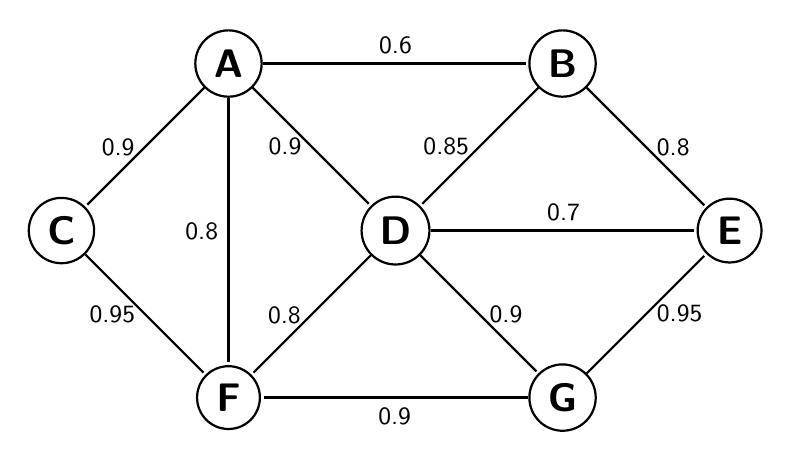
\begin{tikzpicture}[>=stealth',shorten >=1pt,auto,node distance=3cm,
            thick,main node/.style={circle,draw,font=\sffamily\Large\bfseries}]

            %   \node[main node] (1) {1};
            %   \node[main node] (2) [below left of=1] {2};
            %   \node[main node] (3) [below right of=2] {3};
            %   \node[main node] (4) [below right of=1] {4};

            \node[main node] (A) {A};
            \node[main node] (D) [below right of=A]{D};
            \node[main node] (B) [above right of=D]{B};
            \node[main node] (C) [below left of=A]{C};
            \node[main node] (E) [below right of=B]{E};
            \node[main node] (F) [below left of=D]{F};
            \node[main node] (G) [below right of=D]{G};

            \path[every node/.style={font=\sffamily\small}]
            (A) edge node [left] {0.9} (C)
                edge node [left] {0.8} (F)
                edge node [left] {0.9} (D)
                edge node [above] {0.6} (B)
            (B) edge node [left] {0.85} (D)
                edge node [right] {0.8} (E)
            (C) edge node [left] {0.95} (F)
            (D) edge node [above] {0.7} (E)
                edge node [right] {0.9} (G)
                edge node [left] {0.8} (F)
            (G) edge node [below] {0.9} (F)
                edge node [right] {0.95} (E);



            %   \path[every node/.style={font=\sffamily\small}]
            %   (1) edge node [left] {0.6} (4)
            %   edge [bend right] node[left] {0.3} (2)
            %   edge [loop above] node {0.1} (1)
            %   (2) edge node [right] {0.4} (1)
            %   edge node {0.3} (4)
            %   edge [loop left] node {0.4} (2)
            %   edge [bend right] node[left] {0.1} (3)
            %   (3) edge node [right] {0.8} (2)
            %   edge [bend right] node[right] {0.2} (4)
            %   (4) edge node [left] {0.2} (3)
            %   edge [loop right] node {0.6} (4)
            %   edge [bend right] node[right] {0.2} (1);
        \end{tikzpicture}
    \end{center}

\end{homeworkProblem}

%----------------------------------------------------------------------------------------

\end{document}
